%==========================================================================================
\section{Results}\label{sec:dr_results}
%==========================================================================================
Run:
\begin{center}\small\texttt{python scripts/s13\_dynamical\_regimes.py -{}-config configs/md\_unconditional.json}\end{center}
It took 37 minutes. The GPU throttled at 87\,°C, and the $4\times10^5$ clone completions account for 34 of those minutes. Outputs:
\begin{itemize}[nosep]
\item numbers: \texttt{evaluations/md\_unconditional/regimes.json};
\item figures: \texttt{figures/models/md\_unconditional/regimes/}.
\end{itemize}
With 1000 starting points, the standard error of each commitment value is $\le0.01$ (error bars in
Fig.~\ref{fig:dr_spec}).

\subsection{Speciation: a cascade, family first}
\begin{center}\footnotesize
\begin{tabular}{lccccc}
\toprule
 & sibling $D$ & Gaussian law \eqref{eq:ts_mask} & profile Bayes & \multicolumn{2}{c}{cloning with the network}\\
level & (nats) & $k_S$ ($t_S$) & $k_S$ ($t_S$) & (A) true $\bm x_t$: $k_S$ ($t_S$) & (B) own paths: $k_S$ ($t_S$)\\
\midrule
family & 64.5 & 1.6 (0.974) & 2.1 (0.960) & \textbf{2.0} (0.961) & 2.0 (0.962)\\
subfamily & 23.5 & 4.4 (0.927) & 4.9 (0.912) & \textbf{5.7} (0.899) & 5.6 (0.899)\\
clade & 10.4 & 9.8 (0.836) & 8.1 (0.859) & \textbf{16.0} (0.732) & 17.6 (0.700)\\
\bottomrule
\end{tabular}
\end{center}
$k_S$ is the number of revealed sites at which the normalised commitment $\psi$ crosses $1/2$. $t_S$ is the same
crossing for the curve averaged over the binomial number of revealed sites at masking time $t$, eq.~\eqref{eq:k_to_t}.

\begin{figure}[H]
\centering
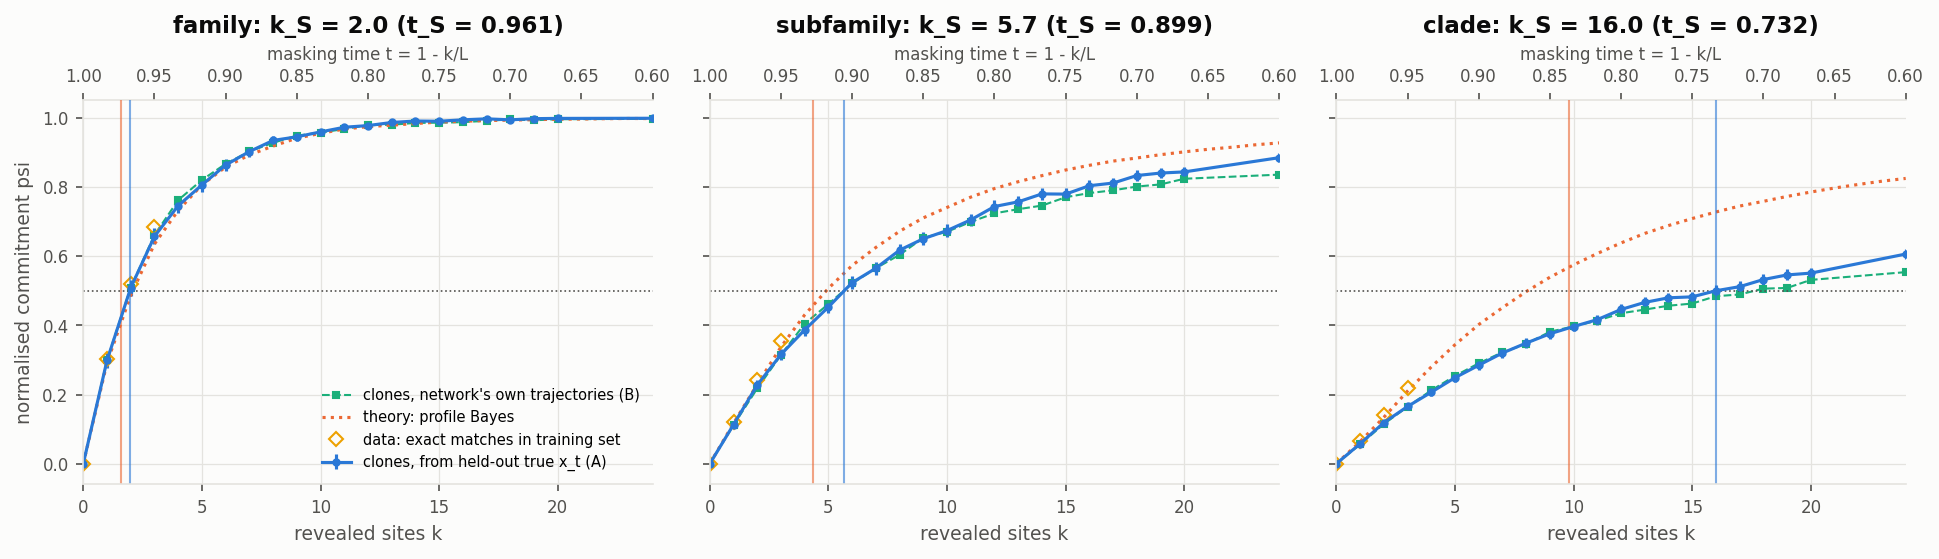
\includegraphics[width=\textwidth]{models/md_unconditional/regimes/speciation.png}
\caption{Speciation at the three levels of the tree. Blue: clone agreement from masked held-out true sequences (A).
Green, dashed: from the network's own trajectories (B). Orange, dotted: the profile-Bayes theory. Yellow diamonds:
the model-free estimate from exact matches in the training set, shown where $\ge90\%$ of the starting points have at
least 20 matches ($k\le3$). Vertical lines: the Gaussian law \eqref{eq:ts_mask} (orange) and the measured $k_S$ (blue).
Top axis: $t=1-k/L$.}
\label{fig:dr_spec}
\end{figure}

\paragraph{The hierarchy is decided top-down.} The family is decided after about \textbf{2 revealed sites}
($t_S=0.96$), the subfamily after about \textbf{6} ($t_S=0.90$), and the clade much later, after about \textbf{16}
($t_S=0.73$). The order follows the sibling divergences $D$, as \eqref{eq:ts_mask} predicts: the more two sibling
classes differ, the fewer residues are needed to tell them apart. The two starting ensembles give the same curves,
as they must for a model whose trajectories are consistent with its own samples (\S\ref{sec:dr_mask_spec}).

\paragraph{Family level: the network is exact.} The three independent estimates agree:
\begin{center}\footnotesize
\begin{tabular}{lccc}
\toprule
$\psi$ at $k=$ & 1 & 2 & 3\\
\midrule
data only (exact matches in the 144\,000 training sequences) & 0.30 & 0.52 & 0.68\\
network clones (A) & 0.30 & 0.51 & 0.66\\
profile Bayes & 0.29 & 0.49 & 0.64\\
\bottomrule
\end{tabular}
\end{center}
With 64.5 nats of class information spread over 60 sites, one revealed residue carries about 1 nat about the family.
Two residues take the commitment halfway, and by $k=10$ it is 0.96.

\paragraph{Subfamily and clade levels: the network commits too slowly.} Here the network's curves lie below both the
data and the theory. At $k=3$ the model-free estimate is 0.36 (subfamily) and 0.22 (clade); the network gives 0.32 and
0.17. Proposition~\ref{prop:clone}(ii) gives an independent check that needs no reference. With the exact denoiser,
two clones agree exactly as often as a clone agrees with the original sequence. For the network:
\begin{center}\footnotesize
\begin{tabular}{lcccccc}
\toprule
 & \multicolumn{2}{c}{family} & \multicolumn{2}{c}{subfamily} & \multicolumn{2}{c}{clade}\\
$k$ & clone--clone & clone--original & clone--clone & clone--original & clone--clone & clone--original\\
\midrule
2 & 0.672 & 0.668 & 0.315 & 0.313 & 0.168 & 0.173\\
5 & 0.871 & 0.879 & 0.515 & 0.529 & 0.290 & 0.317\\
10 & 0.973 & 0.977 & 0.711 & 0.741 & 0.430 & 0.479\\
20 & 0.999 & 0.999 & 0.861 & 0.890 & 0.576 & 0.646\\
\bottomrule
\end{tabular}
\end{center}
(``clone--original'' uses the true label of the original sequence.) At the family level the two columns agree, so
the network behaves like the exact denoiser. At the subfamily and clade levels, clones agree with the original more
than with each other. Write $Q(y\mid\bm x_U)$ for the network's class distribution of completions and $P$ for the
true one. Clone--clone is $\E\sum_yQ^2$ and clone--original is $\E\sum_yPQ$. The second exceeding the first means
that $Q$ is \emph{flatter} than $P$: the network spreads its completions over sibling subfamilies and clades too
evenly. This is the same weakness Part~III found from the other side: within-family correlations about 10\% too weak,
and per-clade $r_C=0.764$ against 0.828 for true samples. The fine-grained, clade-specific structure is learned
only partially, so the network decides the clade late.

\paragraph{Two caveats on the clade value.} (1) Clades genuinely overlap. Even the profile posterior of a
\emph{complete} sequence reaches only $\psi=0.94$, and the classifier that labels the clones is right for 91.5\% of
clades. The clade curve therefore rises slowly towards its ceiling, and its $1/2$-crossing is sensitive: small
changes in the curve move $k_S$ by several sites. (2) The data-only estimate stops at $k=3$, because beyond that most
partial sequences have fewer than 20 exact matches. It is exact where it exists, so the robust statement is: at the
clade level the network is less committed than the data at every $k$ we can check, and its $k_S=16$ is an upper
bound on the true clade speciation. The profile theory places the true value near 8--10.

\begin{figure}[H]
\centering
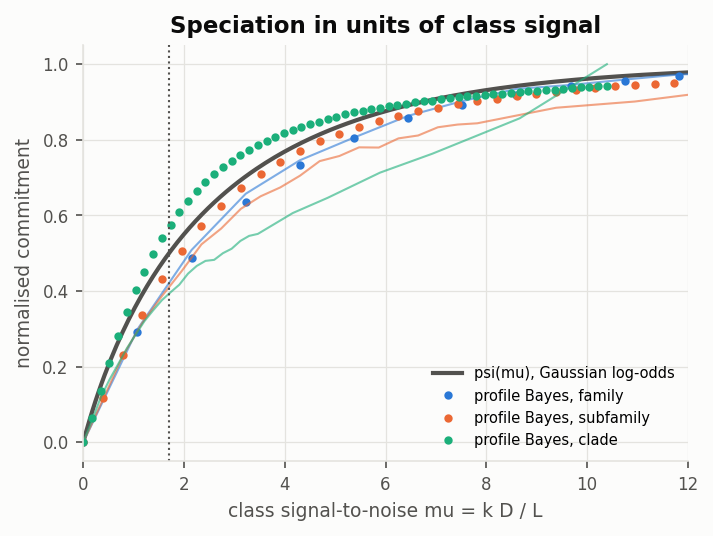
\includegraphics[width=0.46\textwidth]{models/md_unconditional/regimes/speciation_universal.png}\hfill
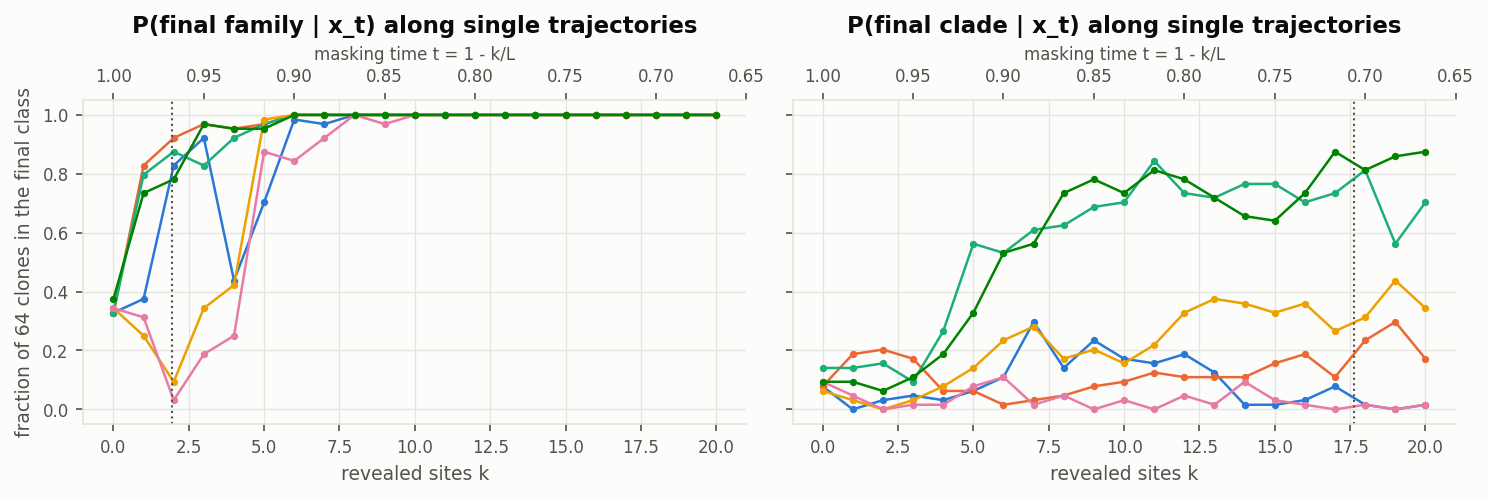
\includegraphics[width=0.52\textwidth]{models/md_unconditional/regimes/trajectories.png}
\caption{Left: the three levels in units of class signal-to-noise $\mu=kD/L$. Dots: profile Bayes. Thin lines:
network clones. Grey: the universal Gaussian curve $\Psi(\mu)$ \eqref{eq:psi_universal}. Right: six single trajectories
of the network, showing at each $k$ the fraction of 64 clones that end in the trajectory's final family (left panel)
or clade (right panel).}
\label{fig:dr_universal}
\end{figure}

\paragraph{One curve for all levels.} Rescaling $k$ by $D/L$ brings the three profile curves close to the single
curve $\Psi(\mu)$ (Fig.~\ref{fig:dr_universal}, left), as the Gaussian argument predicts. The remaining deviations
are expected. At small $\mu$, only a few sites are revealed and $\Lambda$ is a sum of a few non-Gaussian terms. At
large $\mu$ the clades overlap and never fully commit. The network's subfamily and clade curves fall below the
profile ones, which is the under-confidence above.

\paragraph{Single trajectories: symmetry breaking.} Fig.~\ref{fig:dr_universal} (right) is the masked analogue of the
paper's picture of a trajectory falling into one well. The family probability starts at 1/3 and jumps within the
first 2--5 revealed sites. Sometimes it first moves \emph{away} from the final family: the first residues can point
the wrong way, and the next ones correct it. After $k\approx6$ every trajectory is committed. The clade probability
starts at 1/18 and drifts slowly. Two of the six trajectories are clearly committed by $k=10$; the others are still
spread over several clades at $k=20$.

\subsection{Collapse: the quenched theory is exact, the annealed one is not}
\begin{center}\footnotesize
\begin{tabular}{lcc}
\toprule
collapse of the empirical denoiser, $n=144\,000$ & $k_C$ & $t_C$\\
\midrule
measured: $\E[1/N]$ on 1000 trajectories planted on training sequences & \textbf{6.2} & \textbf{0.891}\\
quenched theory \eqref{eq:collapse_mask}, $P(\bm x_U)$ from the network's chain rule & 6.4 & 0.889\\
entropy criterion $H(k_C)=\log n=11.88$ & 6.5 & --\\
annealed theory (collision probability \eqref{eq:collision}) & 10.4 & 0.825\\
\bottomrule
\end{tabular}
\end{center}
\begin{figure}[H]
\centering
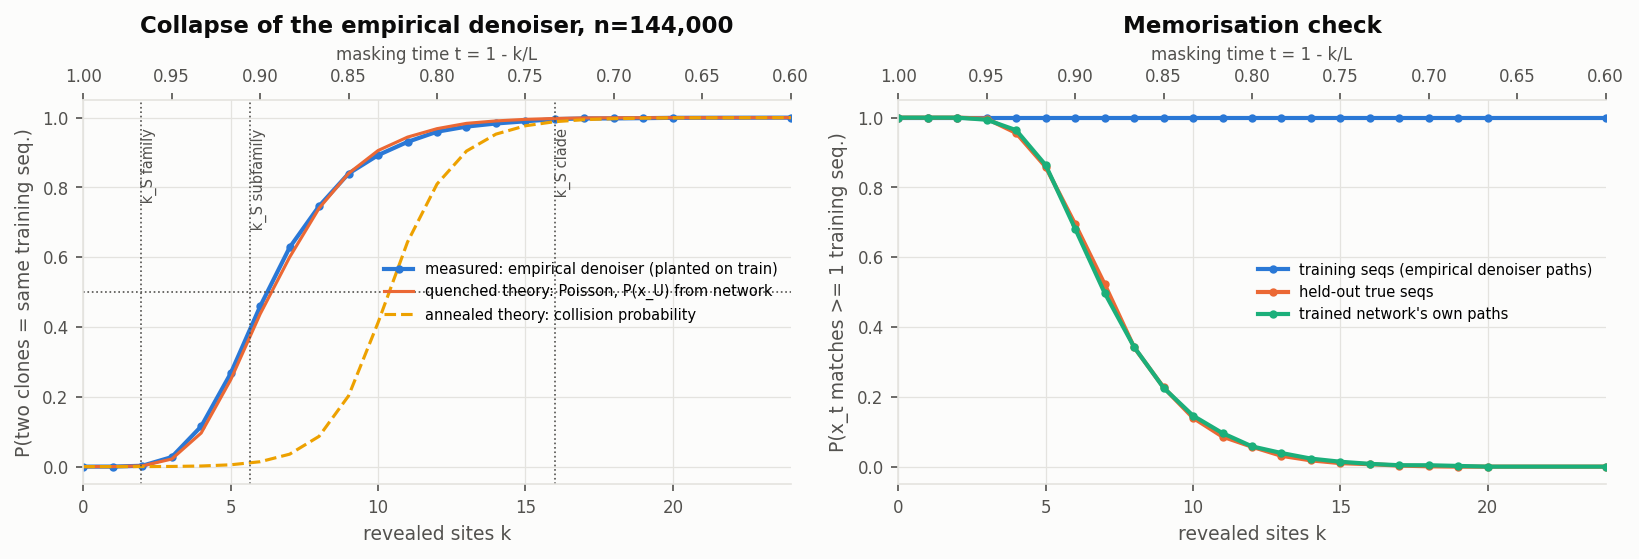
\includegraphics[width=\textwidth]{models/md_unconditional/regimes/collapse.png}
\caption{Left: probability that two clones of the empirical denoiser end on the same training sequence (blue). The
quenched Poisson prediction (orange) follows it at every $k$; the annealed prediction (yellow, dashed) is 4 sites
late. Dotted verticals: the network's speciation times. Right: probability that $\bm x_t$ still agrees with at least one
training sequence, for trajectories planted on training sequences (the empirical denoiser's), held-out true sequences,
and the trained network's own trajectories.}
\label{fig:dr_coll}
\end{figure}
The quenched formula has no fitted parameter. It uses only the network's probabilities of the revealed residues, and
it reproduces the measured collapse curve at every $k$ (Fig.~\ref{fig:dr_coll}, left). The annealed version collapses
4 sites too late. The collision probability is dominated by rare close pairs of training sequences: its entropy
$H_2(k)$ is well below $H(k)$ (Fig.~\ref{fig:dr_entropy}), so it predicts far more matches than a typical trajectory
sees. This is the Random-Energy-Model lesson of \S\ref{sec:dr_gauss_coll} in a setting where it can be checked
exactly.

\paragraph{Collapse versus the number of training sequences.} Measured on random training subsets, and predicted with
the same formula:
\begin{center}\footnotesize
\begin{tabular}{lcccc}
\toprule
$n$ & 100 & 1\,000 & 10\,000 & 144\,000\\
\midrule
$k_C$ measured & 2.12 & 3.38 & 4.70 & 6.43\\
$k_C$ quenched theory & 2.11 & 3.40 & 4.74 & 6.39\\
\bottomrule
\end{tabular}
\end{center}
(The last column repeats the measurement with a different random set of planted sequences: 6.43 against 6.24 above.
This is the size of the sampling noise.)

\begin{figure}[H]
\centering
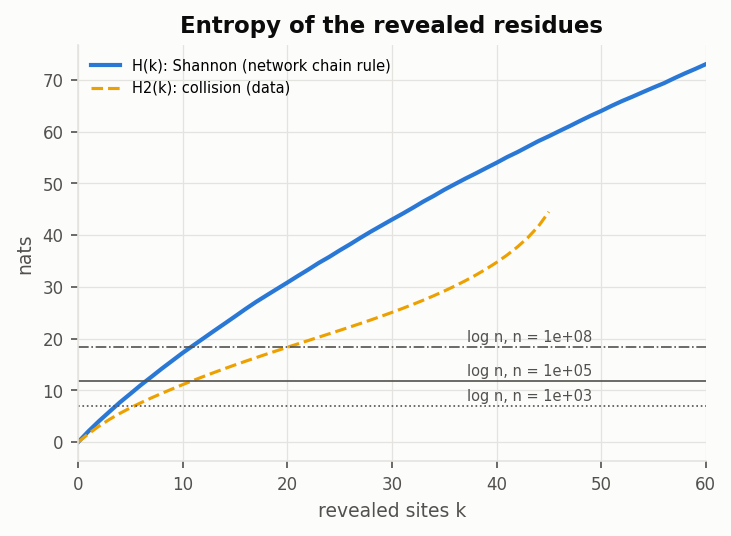
\includegraphics[width=0.46\textwidth]{models/md_unconditional/regimes/entropy.png}\hfill
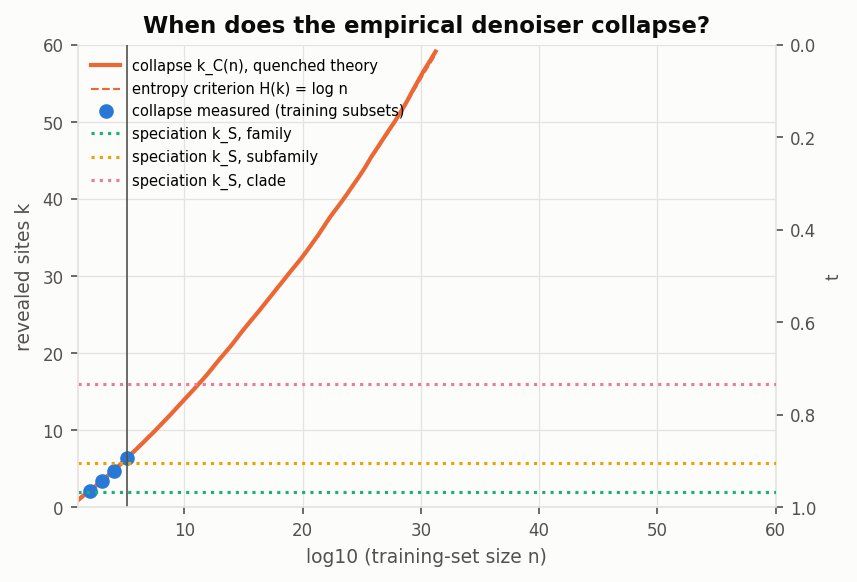
\includegraphics[width=0.5\textwidth]{models/md_unconditional/regimes/phase_diagram.png}
\caption{Left: entropy of the revealed residues. $H(k)$ comes from the network's chain rule; it is 2.1 nats for the
first site and reaches 73.0 nats (1.22 per site, the NELBO) at $k=60$. $H_2(k)$ comes from pairwise Hamming distances. The
collapse happens where $H(k)$ crosses $\log n$. Right: the phase diagram. Collapse $k_C(n)$ (theory line, measured
points) against the three speciation levels. The vertical line marks our $n$.}
\label{fig:dr_entropy}
\end{figure}

\subsection{The three regimes for our data}
For $n=144\,000$, the times of the backward process in order of occurrence are:
\[
\underbrace{k_S^{\rm family}\approx2}_{t=0.96}\;<\;\underbrace{k_S^{\rm subfamily}\approx6}_{t=0.90}\;\lesssim\;
\underbrace{k_C\approx6}_{t=0.89}\;<\;\underbrace{k_S^{\rm clade}\approx8\text{--}16}_{t=0.86\text{--}0.73}.
\]
So the \emph{empirical} denoiser decides the family and, barely, the subfamily before collapsing onto a training
sequence. The clade is never ``speciated'' by it: it is inherited from the memorised sequence. Regimes I, II and III
are cleanly separated only at the family level. The training-set size needed to separate them at level $\ell$ is
$n^\star_\ell=e^{H(k_S^\ell)}$:
\begin{center}\footnotesize
\begin{tabular}{lccc}
\toprule
 & family & subfamily & clade\\
\midrule
$n^\star$ (with the network's $k_S$) & 54 & $3.5\times10^4$ & $1.5\times10^{11}$\\
$n^\star$ (with the profile-Bayes $k_S$) & 68 & $1.0\times10^4$ & $1.6\times10^6$\\
\bottomrule
\end{tabular}
\end{center}
The reason is the entropy scale. One residue carries about 2 nats, so $\log n$ is used up after $\approx6$ residues,
while telling two sibling clades apart takes 8--16. In the paper's language, $\alpha=\log n/L=0.20$ nats per site
is small compared with the entropy per site (1.22 nats). This is the data-poor regime, where the exact minimiser of the
loss memorises early.

\subsection{The trained network does not memorise}
The trained network has the same loss as the empirical denoiser, so the question is how close it gets to that
minimiser. The answer is: not close.
\begin{itemize}[nosep]
\item Along its own trajectories, the probability that $\bm x_t$ still matches a training sequence falls exactly as it
does for \emph{held-out} true sequences (0.50 vs 0.52 at $k=7$, 0.15 vs 0.14 at $k=10$, zero after $k\approx20$). Along
the empirical denoiser's trajectories it stays at 1 (Fig.~\ref{fig:dr_coll}, right). The mean number of matches also
agrees with the held-out value at every $k$ (e.g.\ 24.0 vs 24.6 at $k=7$).
\item Its NELBO is 1.187 nats per site on training sequences and 1.219 on test sequences. That is a gap of 0.03,
against 0.198 (train) and $+\infty$ (test) for the empirical denoiser. The chain-rule entropy of training sequences is
71.5 nats against 73.0 for test sequences. There is a small beginning of preference for training data, far from
memorisation.
\end{itemize}
In the three-regime picture, the network's trajectories pass through regimes I and II and end in regime II. They
never enter regime III. The network generalises although its loss's exact minimiser would collapse after 6 residues.
Generalisation comes from what the network can represent easily and from finite training, not from reaching the
optimum of its loss. (The paper makes the same point for Gaussian diffusion: networks memorise when $n$ is small
compared with their capacity or when they are trained for very long.)

\begin{keybox}{Summary of Part IV}
\begin{itemize}[nosep,leftmargin=*]
\item The two times of Biroli, Bonnaire, de Bortoli and Mézard transpose to masked diffusion with exact
statements. Speciation is the collision probability of the class posterior, measured by cloning. It follows a
universal curve in the class signal-to-noise ratio $\mu$, which for masking is $\mu=(1-t)D$ (for Gaussian noise,
$2\Lambda_{\max}e^{-2t}$). Collapse is $\E[1/N]$, with $N-1$ Poisson-distributed; it happens when the entropy of the
revealed residues reaches $\log n$.
\item Speciation is hierarchical. Family after $\approx2$ residues ($t_S=0.96$), subfamily after $\approx6$ (0.90),
clade after 8--16 (0.86--0.73). At the family level, the network, the data and the theory agree within 0.02.
\item At the subfamily and clade levels the network commits too slowly: its completions are spread too evenly over
sibling classes. This was detected without any reference, by comparing clone--clone with clone--original agreement.
\item The empirical denoiser (the exact optimum of the loss) collapses after 6.2 residues ($t_C=0.89$), between
subfamily and clade speciation. The quenched Poisson theory predicts this to within 0.2 sites for $n$ from $10^2$ to
$1.4\times10^5$; the annealed one is 4 sites late.
\item The trained network does not collapse. Its trajectories leave the training set exactly like held-out data, and its
train/test likelihood gap is 0.03 nats per site.
\end{itemize}
\end{keybox}
